\externaldocument{tech_eclipse_text}

\subsection{Results \label{results}}
The program does a good job of recovering the input brightness values and matching the light curves. The level of noise has some effect on the reproduction of the brightness values, but clear trends can still be seen even with simulated 14th magnitude noise. One important thing to note is that the program does not recover the correct brightness values every time, but does a good job when averaged over many windows. This means that the results are better interpreted as long term trends than as exactly correct in every window. For the synthetic light curves, starspot evolution was not introduced. However, in real systems starspot evolution would exist. This means that our program can give information about overall trends in starspot evolution, but it cannot be trusted to give the exact brightness values of a region for any given time step. 

Further, the algorithm needs at least one full period per window in order to accurately reproduce the box values. With higher noise levels, more of the lightcure must be included at once. There is a tradeoff in lightcurve fit versus avoiding systematics that stem from not having enough information to recover the brightness values. It is counterintuitive to think that the brightness values are recovered more accurately overall the worse the lightcurve fit gets, but this is true. One important thing to note is that the lightcurve fit still fits extremely well overall, but there is more variation from window to window.

In all cases, the light curve fits look good for synthetic curves and real data alike. The fit of the light curve is good irrespective of noise level in the synthetic curve. The RMS of the recovered brightness values is dependent upon the noise levels, but they are still reliably recovered even with simulated 14th magnitude noise.

We have created seven diagnostic plots to compare our synthetic light curve inputs to the model outputs recovered by the code for those same inputs. The first of these plots is the input brightness map shown in Figure~\ref{model_map}. This shows every region on the star and the relative brightness values of each region that was used to create the corresponding synthetic light curve that is then fed into the eclipse mapping code.

\begin{figure}[h]
	\centering
	\includegraphics[width=.5\textwidth]{images/model_map.eps}
	\caption{The set of brightness values used to produce a specific synthetic lightcurve. In this case, this was used to produce the 1b/ set of lightcurves (no noise, 12th magnitude noise, 14th magnitude noise).}
	\label{model_map}
\end{figure}

To visualize the brightness values, we use Figures~\ref{stripe_plot} and~\ref{box_plot}. Along the x-axis is window number defined in Section~\ref{setup}. The y-axis shows the longitude of the star. The top of the plot starts at longitude 0, and the bottom of the plot ends at longitude 360 and then wraps around.These longitudes correspond to the region numbers. This is why we must separate the box and stripe visualizations. The stripes and boxes occupy the same longitude space. Each "pixel's" color is indicative of the brightness value for a given region during a given window. Each vertical strip shows a complete set of box or stripe brightness values for one window. Each horizontal strip shows the recovery for the same region over every window. The value on the far right, beyond the black separator, is the input brightness value for the synthetic light curves. You can compare the recovered brightness in that pixel with all of those in the same region to the left on the same horizontal slice.

\begin{figure}[h]
	\centering
	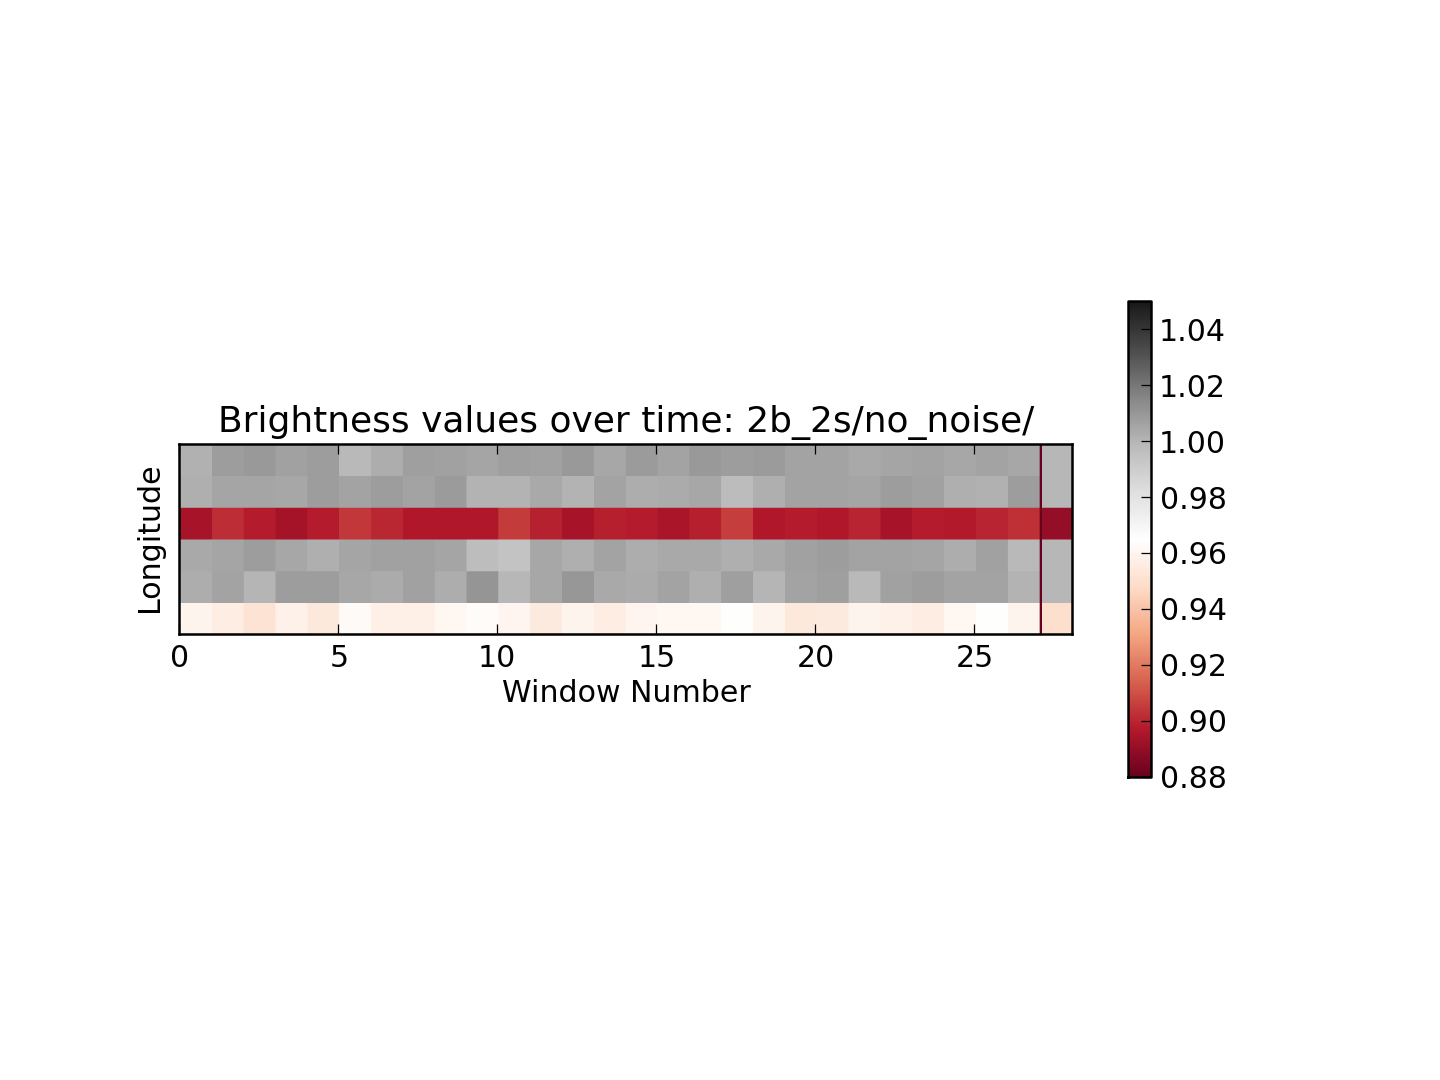
\includegraphics[width=.5\textwidth]{images/stripe_plot.eps}
	\caption{Recovered stripe brightness plot versus window number. This plot is for the no noise model with 1 box darkened. Note the desired values on the far right.}
	\label{stripe_plot}
\end{figure}

\begin{figure}[h]
	\centering
	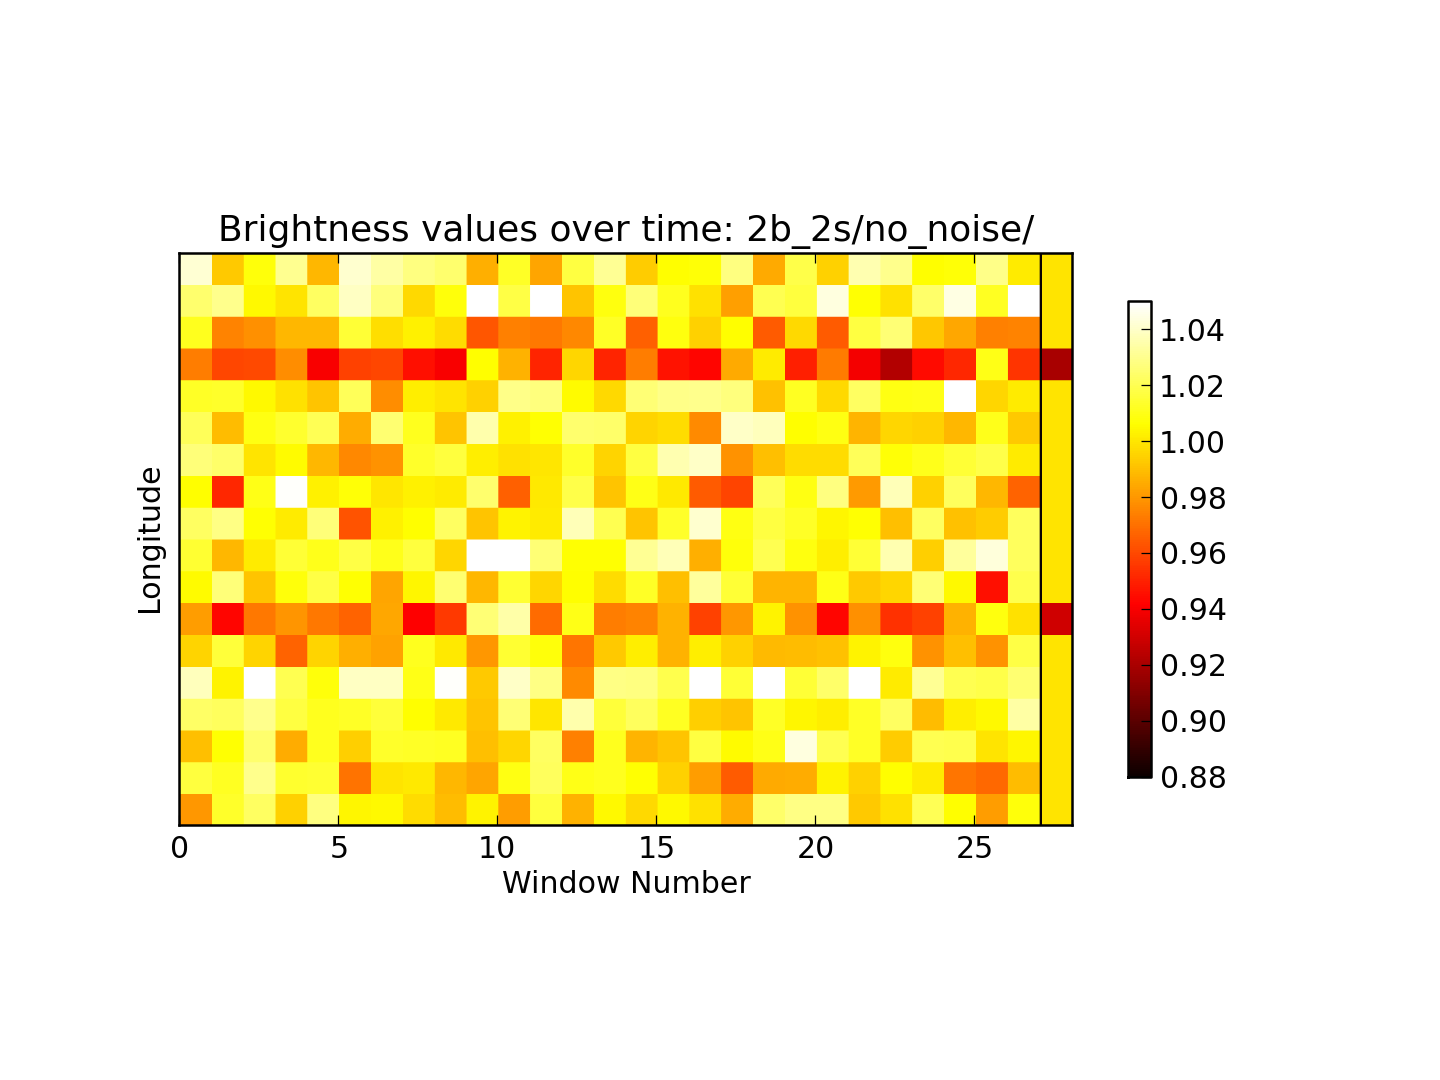
\includegraphics[width=.5\textwidth]{images/box_plot.eps}
	\caption{Recovered box brightness plot versus window number.  This plot is for the no noise model with 1 box darkened. Note the desired values on the far right.}
	\label{box_plot}
\end{figure}

An important thing to note, that should be evident from the discussion of the box and stripe brightness visualizations is that we are working with multiple windows in all cases. This makes it hard to show the brightness recovered for each individual window on the surface of a star in a compact and meaningful way. Because of this, we only show the average brightness recovered over all windows and plot it on the star similar to the input brightness map. You can see this in Figure~\ref{average_map}. For our synthetic lightcurves, this map should match the input map because there is no starspot evolution included. In a real system, a model brightness map is inadequate because evolution could occur. The average over the given time period will be correct, but it will not be reporting all of the information that has been recovered. In this situation, it would be best to produce a separate brightness map for every window or just revert to the box and stripe brightness visualizations shown in Figures~\ref{stripe_plot} and ~\ref{box_plot}.

\begin{figure}[h]
	\centering
	\includegraphics[width=.5\textwidth]{images/average_map.eps}
	\caption{Average brightness value in each region over all windows of an eclipse-mapping code run that was attempting to recover the 1b/no\_noise lightcurve.}
	\label{average_map}
\end{figure}

The next figure is the RMS of the average brightness recovered for a given region over all windows versus the input brightness used to produce the synthetic lightcurve shown in Figure~\ref{rms}. The red diamonds are the regions that have been modified from the default brightness of 1.0. This is only useful to verify that we recover the values used to create our synthetic lightcurves. It has no use for real data because we don't know the brightness values before running the code.

\begin{figure}[h]
	\centering
	\includegraphics[width=.5\textwidth]{images/rms.eps}
	\caption{Comparison of the average value over all windows for each region versus the input value for each region. This particular plot is for the 1b/no\_noise lightcurve.}
	\label{rms}
\end{figure}

The next plot is the lightcurve fit shown in Figure~\ref{lc_fit}. The red points are the input, synthetic lightcurve data. The black lines are the model fits. One thing to note here is that there are actually as many black lines as there are windows. Each black line is overlaid on top of the corresponding portion of lightcurve. As you can see in all cases, it looks like one line, and the fits are incredibly good. 

\begin{figure}[h]
	\centering
	\includegraphics[width=.5\textwidth]{images/lightcurve.eps}
	\caption{Light curve fit of the recovered models versus the synthetic lightcurve. This particular fit has 51 model fits overlaid on top of the red data and is the recovery for the 1b/no\_noise lightcurve.}
	\label{lc_fit}
\end{figure}

The final plot is that of the transit fits. Just like the overall lightcurve fit, there are multiple windows per transit that are being plotted. As the complexity grows, you can see this more and more. Each of these transit pages has the transits in order as you would read in English. We based our synthetic lightcurves off of the third month of Kepler-17 data. This particular data set has 20 transits, so all of our models have exactly 20 transits to recover.
